\documentclass[a4paper,10pt]{article}
\usepackage[brazilian]{babel}
\usepackage[left=2.5cm,right=2.5cm,top=3cm,bottom=2.5cm]{geometry}
\usepackage{mathtools}
\usepackage{amsthm}
\usepackage{amsmath}
%\usepackage{nccmath}
\usepackage{amssymb}
\usepackage{amsfonts}
\usepackage{physics}
%\usepackage{dsfont}
%\usepackage{mathrsfs}

\usepackage{titling}
\usepackage{indentfirst}

\usepackage{bm}
\usepackage[dvipsnames]{xcolor}
\usepackage{cancel}

\usepackage{xurl}
\usepackage[colorlinks=true]{hyperref}

\usepackage{float}
\usepackage{graphicx}
%\usepackage{tikz}
\usepackage{caption}
\usepackage{subcaption}

%%%%%%%%%%%%%%%%%%%%%%%%%%%%%%%%%%%%%%%%%%%%%%%%%%%

\newcommand{\eps}{\epsilon}
\newcommand{\vphi}{\varphi}
\newcommand{\cte}{\text{cte}}

\newcommand{\N}{\mathbb{N}}
\newcommand{\Z}{\mathbb{Z}}
\newcommand{\Q}{\mathbb{Q}}
\newcommand{\R}{\vb{R}}
\newcommand{\C}{\mathbb{C}}
\renewcommand{\S}{\hat{S}}
%\renewcommand{\H}{\s{H}}

\renewcommand{\a}{\vb{a}}
\newcommand{\nn}{\hat{n}}
\renewcommand{\d}{\dagger}
\newcommand{\up}{\uparrow}
\newcommand{\down}{\downarrow}

\newcommand{\0}{\vb{0}}
%\newcommand{\1}{\mathds{1}}
\newcommand{\E}{\vb{E}}
\newcommand{\B}{\vb{B}}
\renewcommand{\v}{\vb{v}}
\renewcommand{\r}{\vb{r}}
\renewcommand{\k}{\vb{k}}
\newcommand{\p}{\vb{p}}
\newcommand{\q}{\vb{q}}
\newcommand{\F}{\vb{F}}

\newcommand{\s}{\sigma}
%\newcommand{\prodint}[2]{\left\langle #1 , #2 \right\rangle}
\newcommand{\cc}[1]{\overline{#1}}
\newcommand{\Eval}[3]{\eval{\left( #1 \right)}_{#2}^{#3}}

\newcommand{\unit}[1]{\; \mathrm{#1}}

\newcommand{\n}{\medskip}
\newcommand{\e}{\quad \mathrm{e} \quad}
\newcommand{\ou}{\quad \mathrm{ou} \quad}
\newcommand{\virg}{\, , \;}
\newcommand{\ptodo}{\forall \,}
\renewcommand{\implies}{\; \Rightarrow \;}
%\newcommand{\eqname}[1]{\tag*{#1}} % Tag equation with name

\setlength{\droptitle}{-7em}

\theoremstyle{plain}
\newtheorem{theorem}{Teorema}[section]
%\newtheorem{defi}[theorem]{Definição}
\newtheorem{lemma}[theorem]{Lema}
%\newtheorem{corol}[theorem]{Corolário}
%\newtheorem{prop}[theorem]{Proposição}
%\newtheorem{example}{Exemplo}
%
%\newtheorem{inneraxiom}{Axioma}
%\newenvironment{axioma}[1]
%  {\renewcommand\theinneraxiom{#1}\inneraxiom}
%  {\endinneraxiom}
%
%\newtheorem{innerpostulado}{Postulado}
%\newenvironment{postulado}[1]
%  {\renewcommand\theinnerpostulado{#1}\innerpostulado}
%  {\endinnerpostulado}
%
%\newtheorem{innerexercise}{Exercício}
%\newenvironment{exercise}[1]
%  {\renewcommand\theinnerexercise{#1}\innerexercise}
%  {\endinnerexercise}
%
%\newtheorem{innerthm}{Teorema}
%\newenvironment{teorema}[1]
%  {\renewcommand\theinnerthm{#1}\innerthm}
%  {\endinnerthm}
%
\newtheorem{innerlema}{Lema}
\newenvironment{lema}[1]
  {\renewcommand\theinnerlema{#1}\innerlema}
  {\endinnerlema}
%
%\theoremstyle{remark}
%\newtheorem*{hint}{Dica}
%\newtheorem*{notation}{Notação}
%\newtheorem*{obs}{Observação}


\title{\Huge{\textbf{Introdução à supercondutividade não-convencional}}}
\author{Mateus Marques}

\begin{document}

\maketitle

\section{Introdução}

Dizemos que um supercondutor é não-convencional quando este não pode ser adequadamente descrito pela teoria BCS (Bardeen-Cooper-Schrieffer). A busca por um mecanismo que explique os diversos tipos de supercondutividade não-convencionais, apesar de antiga, ainda se configura como um dos temas de pesquisa mais importantes dentro da área da Física da Matéria Condensada. Em geral, espera-se que o entendimento da origem dos supercondutores de alta temperatura ajude na procura experimental por um material supercondutor à temperatura ambiente, o que possibilitaria poderosas aplicações tecnológicas, como a transmissão em larga escala de energia elétrica sem dissipação.

Os supercondutores de alta temperatura, especialmente os cupratos, são os mais acessíveis hoje em dia devido ao $T_c$ ser maior que a temperatura de ebulição de $77 \unit{K}$ do nitrogênio líquido, que funciona como um refrigerante relativamente barato.

\begin{figure}[H]
\centering
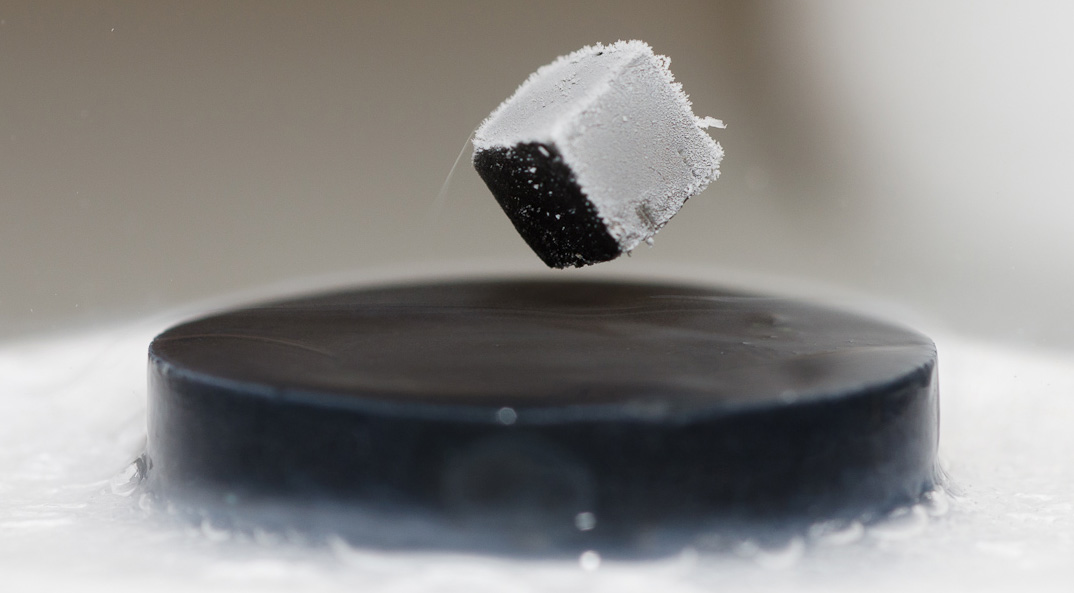
\includegraphics[width=0.7\textwidth]{fig/levitating.jpg}
\caption{Supercondutor de cuprato levitando sobre um ímã pelo efeito Meissner.}
\label{fig:levitating}
\end{figure}

%$$
%U_{\k\k'} =
%\begin{cases}
%\; -g, \text{ se } E_F \leq \eps(\k), \eps(\k') \leq E_F + \hbar \omega_D \\
%\; 0, \text{ caso contrário.}
%\end{cases}
%$$

Existe bastante diversidade dentre todos os supercondutores já conhecidos, e é uma tarefa um pouco arriscada afirmar com exatidão as propriedades de um supercondutor específico, devido a ser um tópico com uma quantidade enorme de pesquisa, discussão e controvérsia dentro da comunidade.

O primeiro supercondutor (convencional) descoberto foi o mercúrio (Hg) em 1911, sendo resfriado por hélio líquido e possuindo $T_c = 4.2 \unit{K}$. Nas décadas subsequentes outros supercondutores foram sendo descobertos, como chumbo (Pb) e nióbio (Nb). Na década de 1930 foi descoberto o efeito Meissner, onde supercondutores tendem a expulsar todo campo magnético aplicado sobre eles. Esse efeito é uma manifestação muito atraente do estado supercondutor, pois permite que vejamos sua ação a olho nu em experimentos relativamente fáceis de fazer, c.f. Figura \ref{fig:levitating}. Na década de 50 foi estabelecida a teoria BCS de supercondutividade, que conseguia explicar todos os supercondutores conhecidos até então. Seus autores John Bardeen, Leon N. Cooper e Robert Schrieffer compartilharam o prêmio Nobel pela teoria BCS em 1972.

Seguindo a referência \cite{timm}Foi na década de 80 que começaram as descobertas de diversos tipos de materiais que aparentemente não conseguiam ser descritos pela teoria BCS, por razões diferentes:
\begin{itemize}
\item Em 1979 foi observado supercondutividade abaixo de $T_c \simeq 0.5 \unit{K}$ no Ce$_2$Cu$_2$Si$_2$, que não tem estado normal de metal, mas sim de um material heavy-fermion, devido às grandes correlações dos elétrons de orbital $f$ do Ce, a massa efetiva do material excede muito a massa do elétron $m^* \ll m_e$.
\item Também em 1979 foi observado supercondutividade em materiais orgânicos.
\item \textbf{Supercondutividade nos cupratos.} The first high-temperature superconductor was discovered in 1986, by IBM researchers Bednorz and Müller,[2][3] who were awarded the Nobel Prize in Physics in 1987 "for their important break-through in the discovery of superconductivity in ceramic materials".[4] Most high-Tc materials are type-II superconductors.
\item Em 1994 descobriram supercondutividade no Sr$_2$RuO$_4$, que por muito tempo pensou que se tratava de uma simetria p-wave, assim como o estado superfluido do $^3$He. Porém experimentos recentes colocam isso em dúvida, mas sua supercondutividade é não-convencional.
\item Em 2001 foi relatado supercondutividade no MgB$_2$ com $T_c = 39 \unit{K}$. Por ser uma temperatura crítica tão alta e o material possuir uma estrutura cristalina parecida dos cupratos, houve a expectativa de ser não-convencional. Porém, acredita-se que na verdade ele seja BCS.
\item Nos anos 2000 foi descoberta uma nova classe de supercondutores baseados em compostos que possuem átomos de ferro, batizados de pnictideos de ferro. Eles são curiosos pois, apesar de possuir átomos de ferro, seus compostos possuem estado com ordem antiferromagnética, mas diferente dos cupratos a maioria deles são metálicos.
\end{itemize}

Na tabela \ref{tab:superconductors} temos



\begin{table}[H]
\begin{center}
\begin{tabular}{ |p{3cm}||p{3cm}|p{3cm}|p{3cm}|  }
\hline
Supercondutor & Simetria & $T_c \simeq$ & Categoria \\
\hline
Hg                   & s-wave   & $4.2   \, \text{K}$      & BCS \\
MgB$_2$              & s-wave   & $39    \, \text{K}$      & BCS \\
$^3$He               & p-wave   & $2.5   \, \text{mK}$     & Superfluido \\
Sr$_2$RuO$_4$        & $-$      & $0.93  \, \text{K}$      & $-$ \\
YBCO                 & d-wave   & $93  \, \text{K}$        & Cuprato \\
BSCCO-2223           & d-wave   & $108   \, \text{K}$      & Cuprato \\
UPt$_3$              & f-wave   & $0.51  \, \text{K}$      & Heavy-Fermion \\
K$_3$C$_{60}$        & $-$      & $18    \, \text{K}$      & Orgânico  \\
LaO$_{1-x}$F$_x$FeAs & $-$      & $26    \, \text{K}$      & Ferro  \\
MATBG                & $-$      & $1.7    \, \text{K}$     & Grafeno  \\
\hline
\end{tabular}
\end{center}
\caption{oi}
\label{tab:superconductors}
\end{table}


Nesta monografia temos como objetivo discutir como generalizar a teoria BCS para entender alguns aspectos fenomenológicos de supercondutores não-convencionais. Em particular, estamos interessados em

Seguiremos very closely o Coleman \cite{coleman}


\begin{itemize}
\item Passar uma ideia introdutória de como generalizar a teoria BCS para estudar a \textbf{fenomenologia} da supercondutividade não-convencional.

\item Entender a distinção básica das diferentes simetrias (jargão) s, p, d, f-wave.

\item Foco específico nos cupratos e na simetria d-wave.
\end{itemize}

%%%%%%%%%%%%%%%%%%%%%%%%%%%%%%%%%%%%%%%%%%%%%%%%%%%%%%%%%%%%%%%%%%%%%%%%%%%%%%%%%%%%%%%%%%%%%%%%%


\begin{section}{Generalizando a teoria BCS}

\begin{itemize}
\item O estado normal é um líquido de Fermi (metal).

\item Elétrons formam pares de Cooper pela interação atrativa mediada por fônons.

\n

\begin{figure}[H]
\centering
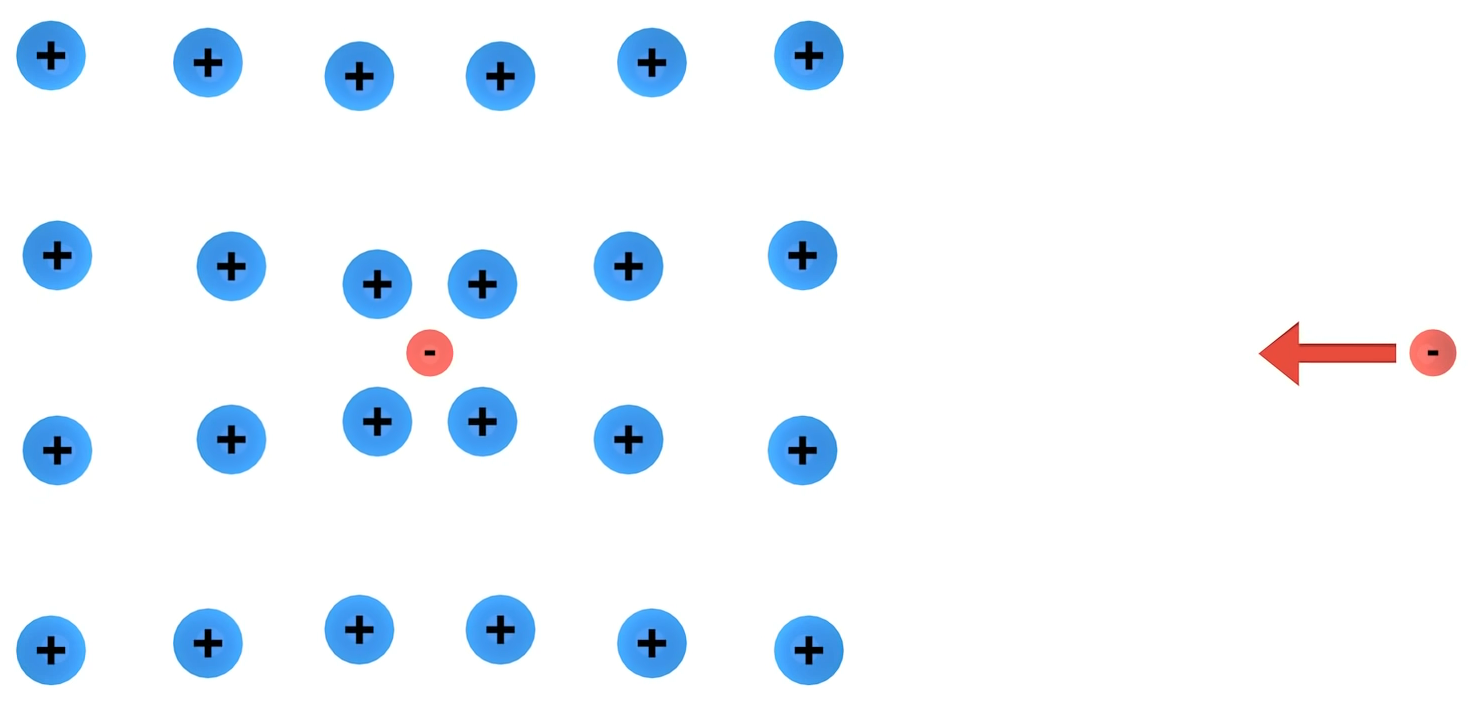
\includegraphics[width=0.5\linewidth]{fig/phonon.png}
\label{fig:phonon}
\end{figure}

\n

\item Os pares de Cooper são bósons e condensam num estado coerente, formando um superfluido carregado.

\item Dispersão $E_{\k} = \sqrt{\eps_{\k}^2 + \abs{\Delta}^2}$, onde o gap $\Delta$ não depende de $\k$ (esfericamente simétrico, ou s-wave).
\end{itemize}

%%%%%%%%%%%%%%%%%%%%%%%%%%%%%%%%%%%%%%%%%%%%%%%%%%%%%%%%%%%%%%%%%%%%%%%%%%%%%%%%%%%%%%%%%%%%%%%%%


Aproveitaremos parte do formalismo da teoria BCS. O raciocínio ainda se baseia na formação de pares de Cooper. Consideremos uma interação do tipo BCS
$$
H_I =
\frac{1}{V} \sum_{\k,\k'} V_{\k,\k'} (c_{\k\up}^\d c_{-\k\down}^\d) (c_{-\k'\down} c_{\k'\up}).
$$

Se definirmos o gap $\Delta_{\k} = \sum_{\k'} V_{\k,\k'} \ev{c_{-\k'\down} c_{\k'\up}}$ e aplicarmos o procedimento de campo médio $AB \simeq A\ev{B} + B\ev{A} - \ev{A}\ev{B}$, generalizamos a equação do gap
\begin{equation} \label{eq:gapeq}
\Delta_{\k} = - \frac{1}{V} \sum_{\k'} V_{\k,\k'} \frac{\Delta_{\k'}}{2 E_{\k'}} \tanh(\frac{\beta E_{\k'}}{2}).
\end{equation}

Devido ao sinal negativo acima, se $V_{\k,\k'}$ não for sempre negativo, a função de gap $\Delta_{\k}$ poderá ser negativa em alguns pontos, de maneira a surgirem nós. Esse fenômeno acontece em várias classes de supercondutores: orgânicos, heavy-fermion, cupratos e baseados em ferro.

%%%%%%%%%%%%%%%%%%%%%%%%%%%%%%%%%%%%%%%%%%%%%%%%%%%%%%%%%%%%%%%%%%%%%%%%%%%%%%%%%%%%%%%%%%%%%%%%%
\end{section}

\begin{section}{Termos de interação}

Tendo em mente que queremos capturar os nós da função de gap, faremos considerações gerais sobre potenciais para estudar como a anisotropia pode surgir. Consideremos dois potenciais, um potencial repulsivo genérico
$$
V = \frac{1}{2} \sum_{\substack{\k_1,\k_2,\q \\ \s, \s'}} V_{\q} c_{\k_1+\q,\s}^\d c_{\k_2+\q,\s'}^\d c_{\k_2,\s'} c_{\k_1,\s},
$$
e um magnético
$$
V_{\text{mag}} = \sum_{i,j} J_{ij} \, \vb{S}_i \vdot \vb{S}_j = \frac{1}{2} \sum_{\q} J_{\q} \, \vb{S}_{-\q} \vdot \vb{S}_{\q}.
$$

\n

Analisaremos primeiro o potencial repulsivo $V$.

%%%%%%%%%%%%%%%%%%%%%%%%%%%%%%%%%%%%%%%%%%%%%%%%%%%%%%%%%%%%%%%%%%%%%%%%%%%%%%%%%%%%%%%%%%%%%%%%%


Como estamos interessados na projeção nos pares de Cooper (momento total zero), consideramos que $\k_1 = -\k_2 = \k'$, $\k_1 + \q = -(\k_2 - \q) = \k$ e $\q = \k - \k'$. A interação resultante geral pode ser separada em termos de acordo com os spins
$$
V_{BCS} = \frac{1}{2} \sum_{\substack{\k,\k' \\ \s, \s'}} V_{\k-\k'} c_{\k\s}^\d c_{-\k\s'}^\d c_{-\k'\s'}c_{\k'\s} =
V_{BCS}^{\up\down} + V_{BCS}^{\up\up} + V_{BCS}^{\down\down}.
$$

Foquemos primeiramente no termo mais familiar
$$
V_{BCS}^{\up\down} = \sum_{\k,\k'} V_{\k-\k'} (c_{\k\up}^\d c_{-\k\down}^\d) (c_{-\k'\down} c_{\k'\up}) =
\sum_{\k,\k'} V_{\k-\k'} \Psi_{\k}^\d \Psi_{\k}.
$$

%%%%%%%%%%%%%%%%%%%%%%%%%%%%%%%%%%%%%%%%%%%%%%%%%%%%%%%%%%%%%%%%%%%%%%%%%%%%%%%%%%%%%%%%%%%%%%%%%

Consideremos as propriedades de paridade $P$ e spin exchange $X$ da função de onda $F(\k)_{\alpha\beta} = \braket{\k\alpha,-\k\beta}{\k_P}$ do par de Cooper, definidas por
$$
P F(\k)_{\alpha\beta} = F(-\k)_{\alpha\beta},
$$
$$
X F(\k)_{\alpha\beta} = F(\k)_{\beta\alpha}.
$$

O operador de troca de spin distingue singletos $X = -1$ de tripletos $X = +1$.

\n

Obs: Lembremos que um par de spins $\ket{\up\down}$ não é singleto nem tripleto. De fato, o singleto é $(\ket{\up\down} - \ket{\down\up})/\sqrt{2}$ e o tripleto é composto por $(\ket{\up\down} + \ket{\down\up})/\sqrt{2}$, $\ket{\up\up}$ e $\ket{\down\down}$.

\n

Se aplicarmos $X$ e $P$ em $\braket{\k\alpha,-\k\beta}{\k_P}$ estaremos trocando os dois férmions que compõem o par, adquirindo uma fase $-1$. Portanto, $XP = -1$ no subespaço dos pares de Cooper.

\n

Temos então que pares com paridade par são singletos $(P,X) = (+, -)$ e com paridade ímpar são tripletos $(P,X) = (-,+)$.

%%%%%%%%%%%%%%%%%%%%%%%%%%%%%%%%%%%%%%%%%%%%%%%%%%%%%%%%%%%%%%%%%%%%%%%%%%%%%%%%%%%%%%%%%%%%%%%%%

Com autovalores dos operadores $P$ e $X$ em mente, podemos decompor a interação em partes simétrica (par, singleto) e antissimétrica (ímpar, tripleto):
$$
V_{BCS}^{\up\down} = \sum_{\k,\k'}
\Bigg[
\overbrace{\qty(\frac{V_{\k-\k'} + V_{\k+\k'}}{2})}^{V_{\k,\k'}^S} +
\overbrace{\qty(\frac{V_{\k-\k'} - V_{\k+\k'}}{2})}^{V_{\k,\k'}^T}
\Bigg] \Psi_{\k}^\d \Psi_{\k}.
$$

O primeiro termo acima espalha singletos e o segundo tripletos, representados por
$$
\Psi_{\k}^{S\d} = (c_{\k\up}^\d c_{-\k\down}^\d + c_{-\k\up}^\d c_{\k\down}^\d),
\quad \Psi_{\k}^{S\d} = +\Psi_{-\k}^{S\d},
$$
$$
\Psi_{\k}^{T\d} = (c_{\k\up}^\d c_{-\k\down}^\d - c_{-\k\up}^\d c_{\k\down}^\d),
\quad \Psi_{\k}^{T\d} = -\Psi_{-\k}^{T\d}.
$$

E escrevemos
$$
V_{BCS}^{\up\down} =
\frac{1}{4} \sum_{\k,\k'}
\qty[
V_{\k,\k'}^S \Psi_{\k}^{S\d} \Psi_{\k'}^{S} +
V_{\k,\k'}^T \Psi_{\k}^{T\d} \Psi_{\k'}^{T}
].
$$

%%%%%%%%%%%%%%%%%%%%%%%%%%%%%%%%%%%%%%%%%%%%%%%%%%%%%%%%%%%%%%%%%%%%%%%%%%%%%%%%%%%%%%%%%%%%%%%%%

Os outros termos $V_{BCS}^{\up\up}$ e $V_{BCS}^{\down\down}$ somente envolvem tripletos, que interagem via $V_{\k,\k'}^T$. Se definirmos o vetor tripleto
$$
\va*{\Psi}_{\k}^T = \sum_{\alpha\beta} c_{\k\alpha}^\d \qty(\va*{\s} i \s_2)_{\alpha\beta} c_{-\k\beta}^\d =
\begin{cases}
\; \; \; \; c_{\k\down}^\d c_{-\k\down} - c_{\k\up}^\d c_{-\k\up}^\d \; , \quad (x) \\
\; i (c_{\k\down}^\d c_{-\k\down} + c_{\k\up}^\d c_{-\k\up}^\d), \quad (y) \\
\; \; \; \; c_{\k\up}^\d c_{-\k\down}^\d + c_{-\k\up}^\d c_{\k\down}^\d \; , \quad (z),
\end{cases}
$$
podemos representar as interações de spins paralelos de maneira compacta. No final obtemos
$$
V_{BCS} =
V_{BCS}^{\up\down} + V_{BCS}^{\up\up} + V_{BCS}^{\down\down} =
\frac{1}{4} \sum_{\k,\k'}
\qty(
V_{\k,\k'}^S \Psi_{\k}^{S\d} \Psi_{\k'}^S +
V_{\k,\k'}^T \va*{\Psi}_{\k}^{T\d} \va*{\Psi}_{\k'}^T
).
$$

%%%%%%%%%%%%%%%%%%%%%%%%%%%%%%%%%%%%%%%%%%%%%%%%%%%%%%%%%%%%%%%%%%%%%%%%%%%%%%%%%%%%%%%%%%%%%%%%%


\begin{itemize}
\item Ao estudarmos os harmônicos esféricos $Y_{\ell m}$ no contexto do átomo de Hidrogênio, vemos que a paridade está associada ao número quântico de momento angular orbital $\ell$, de maneira que $Y_{\ell m}(-\r) = (-1)^\ell Y_{\ell m}(\r)$.

\n

\item Pares de Cooper com função de onda de singleto envolvem $\ell = 0, 2, \ldots$ (s, d, $\ldots$ wave) e de tripleto envolvem valores ímpares $\ell = 1, 3, \ldots$ (p, f, $\ldots$ wave).

\begin{figure}[H]
\centering
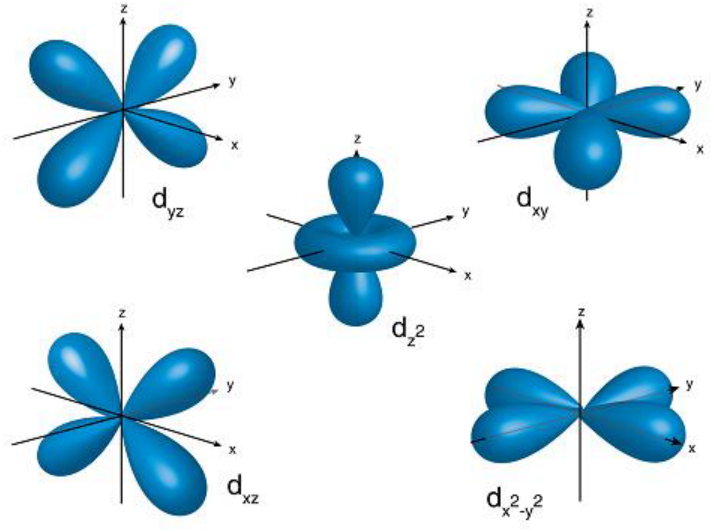
\includegraphics[width=0.27\linewidth]{fig/d-orbitals.png}
\caption{Harmônicos esféricos $Y_{2m}$ dos orbitais $d$.}
\label{fig:d-orbitals}
\end{figure}

\item Já que o potencial repulsivo $V_{BCS}$ se dissocia em interações de singleto e tripleto, podemos estudá-las separadamente. Em especial, só precisamos considerar o termo de tripleto $V^T_{\k,\k'}$ se estivermos interessados em descrever supercondutividade p-wave ou f-wave, por exemplo.

\n

\item Para um acoplamento somente de singleto, ficamos com a familiar
$$
V_{BCS} = \sum_{\k,\k'} V_{\k,\k'}^S (c_{\k\up}^\d c_{-\k\down}^\d) (c_{-\k'\down} c_{\k'\up}).
$$
\end{itemize}

%%%%%%%%%%%%%%%%%%%%%%%%%%%%%%%%%%%%%%%%%%%%%%%%%%%%%%%%%%%%%%%%%%%%%%%%%%%%%%%%%%%%%%%%%%%%%%%%%

Analisemos agora a interação magnética (do tipo Heisenberg)
$$
V_{\text{mag}} = \frac{1}{2} \sum_{\q} J_{\q} \, \va*{S}_{-\q} \vdot \va*{S}_{\q} =
\frac{1}{2} \sum_{\substack{\k_1,\k_2,\q \\ \alpha\beta\gamma\delta}} J_{\q} c_{\k_1+\q,\alpha}^\d c_{\k_2-\q,\gamma}^\d
\qty(\frac{\va*{\s}}{2})_{\alpha\beta} \qty(\frac{\va*{\s}}{2})_{\gamma\delta} c_{\k_2\delta} c_{\k_1\beta},
$$
onde $J_{\q}$ é a interação efetiva dos spins. Por exemplo, para spins em uma rede quadrada interagindo só com primeiros vizinhos temos $J_{\q} = 2 J [\cos(q_x a) + \cos(q_y a)]$ (tight-binding).

\n

Considerando o produto escalar $\qty(\frac{\va*{\s}}{2})_{\alpha\beta} \cdot \qty(\frac{\va*{\s}}{2})_{\gamma\delta} \equiv \va*{S}_1 \vdot \va*{S}_2$, lembremos que seus autovalores são $+\frac{1}{4}$ para o tripleto e $-\frac{3}{4}$ para o singleto (lembre da estrutura hiperfina do hidrogênio):
$$
\va*{S}_1 \vdot \va*{S}_2 =
\begin{cases}
\; +\frac{1}{4} \quad \text{(tripleto)}, \\
\; -\frac{3}{4} \quad \text{(singleto)}.
\end{cases}
$$

%%%%%%%%%%%%%%%%%%%%%%%%%%%%%%%%%%%%%%%%%%%%%%%%%%%%%%%%%%%%%%%%%%%%%%%%%%%%%%%%%%%%%%%%%%%%%%%%%


Já que as partes simétricas e antissimétricas da interação filtram os pares singleto e tripleto, temos que esses autovalores entram como prefatores no potencial, de maneira que
$$
V_{\k,\k'}^S = -\frac{3}{4} \qty(\frac{J_{\k-\k'} + J_{\k+\k'}}{2}), \quad
V_{\k,\k'}^T = +\frac{1}{4} \qty(\frac{J_{\k-\k'} - J_{\k+\k'}}{2}).
$$

Interações antiferromagnéticas ($J > 0 \implies V_{\k,\k'}^S < 0$) causam uma interação atrativa nos pares de singleto e interações ferromagnéticas ($J < 0 \implies V_{\k,\k'}^T < 0$) causam interação atrativa nos pares de tripleto.
$$
\begin{cases}
\; \text{interação antiferromagnética} \leftrightarrow \text{pares singleto anisotrópicos (d-wave),} \\
\; \text{interação ferromagnética} \leftrightarrow \text{pares tripleto anisotrópicos (p-wave).}
\end{cases}
$$

A saber, o estado normal dos cupratos é em geral um isolante de Mott com ordem antiferromagnética. No resto de nossa discussão daremos foco especial a eles.

\end{section}

%%%%%%%%%%%%%%%%%%%%%%%%%%%%%%%%%%%%%%%%%%%%%%%%%%%%%%%%%%%%%%%%%%%%%%%%%%%%%%%%%%%%%%%%%%%%%%%%%


\begin{section}{Cupratos}

\begin{figure}
\centering
   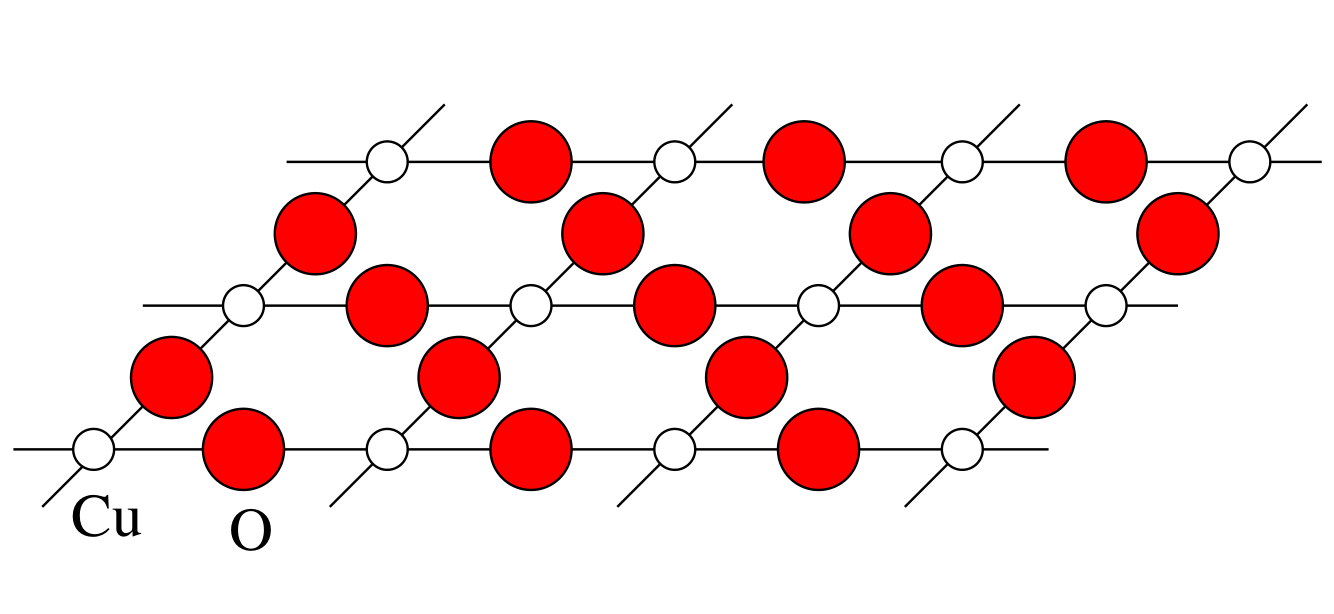
\includegraphics[width=0.475\textwidth]{fig/cuo2.png}
   \quad \quad
   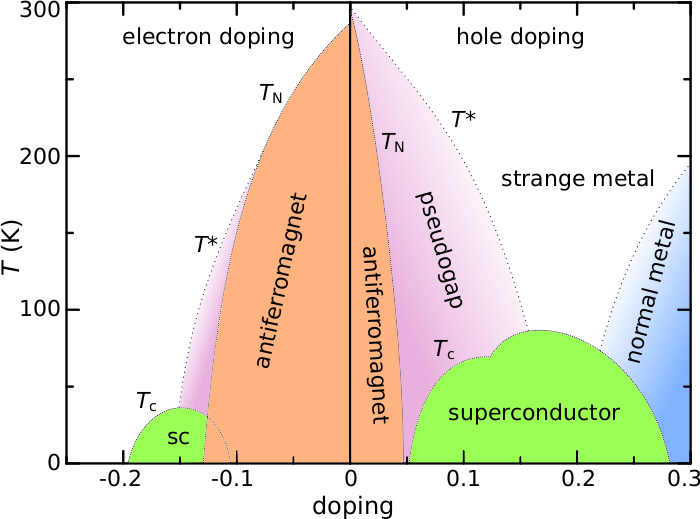
\includegraphics[width=0.32\textwidth]{fig/cuprate-phasediag.png}
   \caption{Propriedades gerais dos cupratos}
\end{figure}


\begin{minipage}[b]{0.75\textwidth}
  \begin{itemize}
  \item Os cupratos consistem de várias camadas de CuO$_2$, que possui uma rede quadrada.
  \item Seu estado normal é um isolante de Mott com ordem antiferromagnética.
  \item A interação atrativa elétron-elétron não é causada por fônons, mas sim por interação antiferromagnética, capaz de gerar supercondutividade d-wave.
  \item Do lado direito do diagrama (superdopado) eles se comportam como líquido de Fermi. Essa é a nossa justificativa para aplicarmos fenomenologia BCS.
  \end{itemize}
\end{minipage}

\begin{figure}[H]
\centering
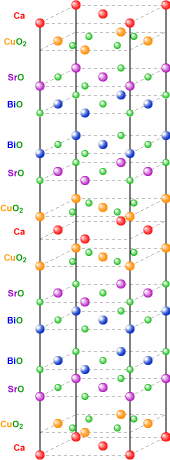
\includegraphics[width=0.2\textwidth]{fig/bscco-unitcell.png}
\caption{Célula unitária BSCCO.}
\label{fig:bscco-unitcell}
\end{figure}

%%%%%%%%%%%%%%%%%%%%%%%%%%%%%%%%%%%%%%%%%%%%%%%%%%%%%%%%%%%%%%%%%%%%%%%%%%%%%%%%%%%%%%%%%%%%%%%%%%%

Consideramos um modelo simplificado de um supercondutor d-wave para os cupratos, onde os elétrons se movem em uma rede quadrada com dispersão $\eps_{\k} = -2t (\cos k_x a + \cos k_y a)$. Incluimos a repulsão de Coulomb por meio de um termo de Hubbard e também consideramos interações antiferromagnéticas para primeiros vizinhos:
$$
H = \sum_{\k} \eps_{\k} c_{\k\s}^\d c_{\k\s} + \sum_{j} U n_{j\up} n_{j\down} + J \sum_{\nn{i}{j}} \va*{S}_i \vdot \va*{S}_j.
$$

Supondo que $U, J \ll t$, tratamos o material como um líquido de Fermi com uma interação BCS de singleto
$$
V^{\text{singleto}}(\q) = U - \frac{3J}{2} (\cos q_x a + \cos q_y a),
$$
onde o fator $-\frac{3}{2}$ surgiu daquele $-\frac{3}{4}$ da discussão anterior.

A interação $V_{\k,\k'}$ é obtida a partir da simetrização
$$
V_{\k,\k'} = \frac{1}{2}
\Big[
V^{\text{singleto}}(\k-\k') + V^{\text{singleto}}(\k+\k')
\Big] =
U - \frac{3}{2} (c_x c_{x'} + c_y c_{y'}),
$$
onde denotamos $c_x = \cos(k_x a)$ e $c_y = \cos(k_y a)$. A hamiltoniana BCS é então
$$
H_{BCS} = \sum_{\k\s} \eps_{\k} c_{\k\s}^\d c_{\k\s} +
\sum_{\k,\k'} \qty[U - \frac{3}{2} (c_x c_{x'} + c_y c_{y'})]
c_{\k\up}^\d c_{-\k\down}^\d c_{-\k'\down} c_{\k'\up}.
$$

%%%%%%%%%%%%%%%%%%%%%%%%%%%%%%%%%%%%%%%%%%%%%%%%%%%%%%%%%%%%%%%%%%%%%%%%%%%%%%%%

Podemos separar a interação $V_{\k,\k'} = V_{\k,\k'}^s + V_{\k,\k'}^d$ em um termo s-wave e d-wave:
$$
V_{\k,\k'}^s =
\overbrace{U}^{\text{s-wave}} -
\overbrace{\frac{3}{4} J (c_x + c_y) (c_{x'} + c_{y'})}^{\text{s-wave estendida}}
\quad \text{(s-wave)},
$$
$$
V_{\k,\k'}^d = - \frac{3}{4} J (c_x - c_y) (c_{x'} - c_{y'})
\quad \text{(d-wave)},
$$
onde o termo s-wave é invariante por rotações de $90^\circ$ e o termo d-wave troca de sinal, $V_{\k,\k'}^s = + V_{\k, R\k'}^s$ e $V_{\k,\k'}^d = - V_{\k, R\k'}^d$ com $R\k = (-k_y, k_x)$.

\n

Se analisarmos a equação \ref{eq:gapeq} do gap
$$
\Delta_{\k} = - \int \frac{\dd[2]{\k'}}{(2\pi)^2} (V_{\k,\k'}^s + V_{\k,\k'}^d) \frac{\Delta_{\k'}}{2 E_{\k'}} \tanh(\frac{\beta E_{\k'}}{2}),
$$
é possível escrever também $\Delta_{\k} = \Delta_{\k}^s + \Delta_{\k}^d$, com
$$
\Delta_{\k}^s = \Delta_1 + \Delta_ 2 (c_x + c_y) = + \Delta_{R\k}^s,
$$
$$
\Delta_{\k}^d = \Delta_d (c_x - c_y) = - \Delta_{R\k}^d.
$$

Os dois termos $\Delta_{\k,\k'}^s$ e $\Delta_{\k,\k'}^d$ se acoplam somente com as respectivas interações s-wave e d-wave na equação do gap, pois $\int \frac{\dd[2]{\k'}}{(2\pi)^2} V_{\k,\k'}^s \Delta^d_{\k'} (\ldots) = 0$ e $\int \frac{\dd[2]{\k'}}{(2\pi)^2} V_{\k,\k'}^d \Delta^s_{\k'} (\ldots) = 0$, devido às integrais mudarem de sinal sob uma rotação de $90^\circ$ e, portanto, serem nulas. Concluimos que as duas simetrias s-wave e d-wave são desacopladas e, em particular, a simetria d-wave é ortogonal ao potencial de Coulomb local $U$.


%%%%%%%%%%%%%%%%%%%%%%%%%%%%%%%%%%%%%%%%%%%%%%%%%%%%%%%%%%%%%%%%%%%%%%%%%%%%%%%%

\n

Analisando o gap d-wave $\Delta_{\k}^d = \Delta_d (c_x - c_y)$, vemos que ele possui nós nas diagonais $k_x = \pm k_y$, de maneira que essa simetria d-wave tem a forma do orbital $d_{x^2-y^2}$ da Figura \ref{fig:d-orbitals}. A energia das quasepartículas $E_{\k} = \sqrt{\eps_{\k}^2 + \Delta_d^2 (c_x - c_y)^2}$ se anula na interseção dessas diagonais (onde $\Delta_{\k} = 0$) com a superfície de Fermi (onde $\eps_{\k} = 0$), de maneira a formar cones de Dirac nesses pontos (nodais), ilustrados na Figura \ref{fig:fermisurf}:

\begin{figure}[H]
\centering
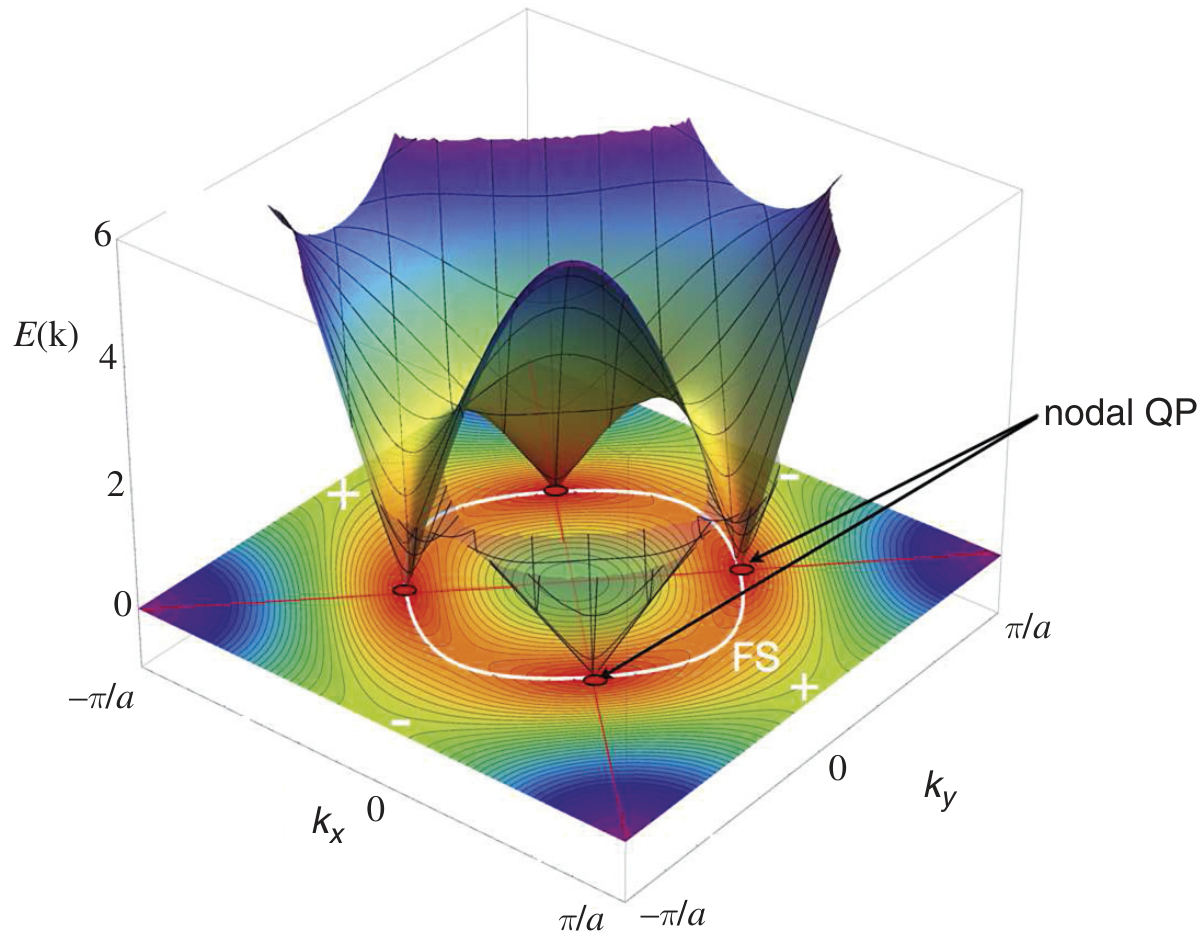
\includegraphics[width=0.45\linewidth]{fig/fermisurf.png}
\caption{Cones de Dirac nos pontos nodais, que se localizam na interseção da superfície de Fermi (FS) com as retas $k_x = \pm k_y$.}
\label{fig:fermisurf}
\end{figure}


%%%%%%%%%%%%%%%%%%%%%%%%%%%%%%%%%%%%%%%%%%%%%%%%%%%%%%%%%%%%%%%%%%%%%%%%%%%%%%%%

Utilizando a equação do gap, podemos fazer algumas aproximações para ter uma ideia da física envolvida. Supondo que o preenchimento ao redor de $\Gamma (\k = \0)$ seja pequeno, temos $\eps_{\k} = -2t (c_x + c_y) \simeq -4t  + t k^2$ e o gap
$$
\Delta_{\k}^d = \Delta_d (c_x - c_y) \simeq -\frac{\Delta_d}{2 k_F^2}
\qty[\qty(\frac{k_x}{k_F})^2 - \qty(\frac{k_y}{k_F})^2] = - \Delta_0 \cos(2\theta),
\quad \Delta_0 = \frac{\Delta_d}{2 k_F^2}, \k = (k_x, k_y) = \abs{\k} e^{i\theta}.
$$
Perceba que $\Delta^d(\theta) \propto \cos(2\theta)$ remete ao harmônico esférico do orbital $d_{x^2 - y^2}$.

\n

Colocando um cutoff na energia $\abs{\eps} \leq \omega_0$ e assumindo que a densidade de estados por spin seja constante $\rho(E_F) = \frac{1}{4\pi t}$, obtemos a equação do gap:
$$
1 = \frac{3 J}{4} \rho(E_F) \int_{-\omega_0}^{\omega_0} \dd{\eps}
\int_0^{2\pi} \frac{\dd{\theta}}{2\pi} \cos[2](2\theta) \frac{\tanh(\frac{\beta E}{2})}{2E}, \quad E = \sqrt{\eps^2 + [\Delta_0 \cos(2\theta)]^2}.
$$

Aproximando grosseiramente $\cos[2](2\theta)$ pela sua média $1/2$, chegamos numa equação aproximada (similar à BCS) para $T_c$:
$$
1 = \frac{3J}{8} \rho(E_F) \int_0^{\omega_0} \dd{\eps} \,
\frac{\tanh(\frac{\eps}{2T_c})}{\eps},
$$
onde é possível obter $T_c \sim 1.13 \, \omega_0 e^{-\frac{8}{3 J \rho(E_F)}}$.


%%%%%%%%%%%%%%%%%%%%%%%%%%%%%%%%%%%%%%%%%%%%%%%%%%%%%%%%%%%%%%%%%%%%%%%%%%%%%%%%

Também podemos calcular a densidade de estados aproximada tomando uma média sobre o ângulo $\theta$:
$$
\frac{N_d(E)}{N(0)} = \dv{\eps}{E} =
\Re{\int_0^{2\pi} \frac{\dd{\theta}}{2\pi}
\frac{\abs{E}}{\sqrt{(E - i\delta)^2 + [\Delta_0 \cos(2\theta)]^2}}
},
$$
em que obtemos a Figura \ref{fig:dwavedos}:

\begin{figure}[H]
\centering
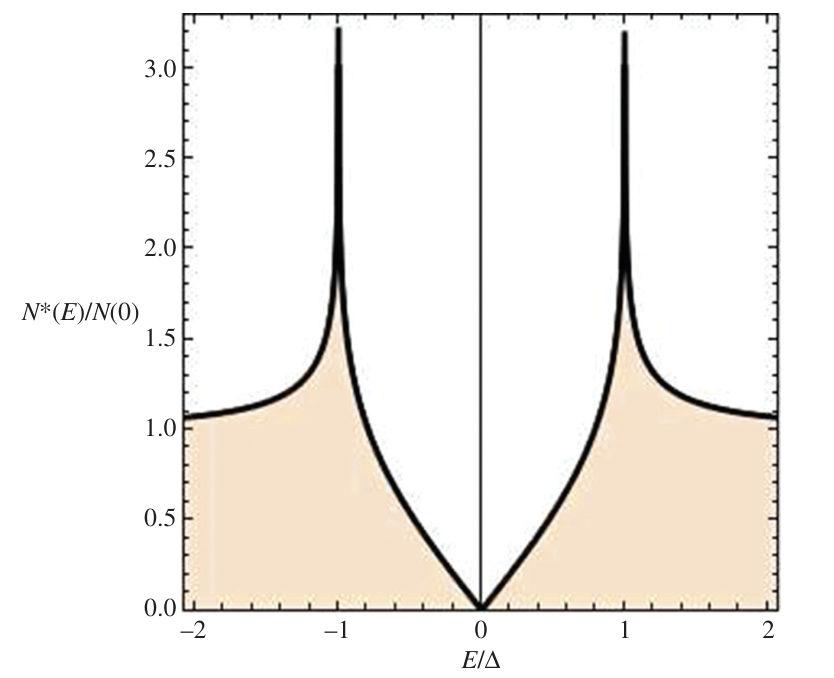
\includegraphics[width=0.25\textwidth]{fig/dwavedos.png}
\caption{Densidade de estados $N_d(E)/N(0)$ aproximada para um supercondutor d-wave.}
\label{fig:dwavedos}
\end{figure}

Note que não temos mais uma densidade de estados gapeada, pois de fato há cones de Dirac pelos nós nas diagonais $k_x = \pm k_y$. A Figura \ref{fig:dwavedos} na verdade parece muito com a DOS do grafeno.

%%%%%%%%%%%%%%%%%%%%%%%%%%%%%%%%%%%%%%%%%%%%%%%%%%%%%%%%%%%%%%%%%%%%%%%%%%%%%%%%

Exploremos por final a componente s-wave do gap $\Delta_{\k}^s = \Delta_1 + \Delta_2 (c_x + c_y)$. A equação do gap correspondente é
$$
\Delta_{\k}^s = - \int \frac{\dd[2]{\k'}}{(2\pi)^2}
\overbrace{\qty[U - \frac{3}{4} J (c_x + c_y)(c_{x'}+ c_{y'})]}^{V_{\k,\k'}^s}
\frac{\Delta_{\k'}^s}{2 E_{\k'}} \, \tanh(\frac{\beta E_{\k'}}{2}).
$$

Ela é mais complicada pois existe acoplamento entre o termo local $\Delta_1$ e o termo s-wave estendido $\Delta_2 (c_x + c_y)$.

\n

De forma simplificada, assumindo uma única superfície de Fermi, um cutoff $\abs{\eps} \leq \omega_0$ e expandindo $\k, \k' \ll t$ próximo do ponto $\Gamma$ de maneira que $c_x \simeq c_y \simeq 1$, temos que a interação efetiva é da ordem de $V_{\k,\k'}^s \simeq U - 3J$.
\n

Isso indica que, para uma única superfície de Fermi, a atração s-wave estendida é suprimida pela interação de Coulomb $U$. Isso faz com que a interação efetiva seja reduzida.

\n

Pensando na fórmula da temperatura crítica BCS para a componente s-wave $T_c^s \sim 1.13 \, \omega_0 e^{-\frac{1}{g \rho(E_F)}}$, essa redução na constante efetiva de acoplamento $g \sim V_{\k,\k'}^s \simeq U-3J$ faz com que a temperatura crítica s-wave diminua.

\n

Essas estimativas indicam que nos cupratos o $T_c^d$ da componente d-wave é maior que $T_c^s$ (que foi suprimido por $U$), fazendo com que o pareamento d-wave seja predominante.

\end{section}


\pagebreak


\section{Fatos aleatórios}

From \url{https://en.wikipedia.org/wiki/Cuprate_superconductor}

\textbf{Introcution Section}

Cuprate superconductors are a family of high-temperature superconducting materials made of layers of copper oxides (CuO2) alternating with layers of other metal oxides, which act as charge reservoirs.

\textbf{Structure Section}

Cuprates are layered materials, consisting of superconducting planes of copper oxide, separated by layers containing ions such as lanthanum, barium, strontium, which act as a charge reservoir, doping electrons or holes into the copper-oxide planes. Thus the structure is described as a superlattice of superconducting CuO2 layers separated by spacer layers, resulting in a structure often closely related to the perovskite structure. Superconductivity takes place within the copper-oxide (CuO2) sheets, with only weak coupling between adjacent CuO2 planes, making the properties close to that of a two-dimensional material. Electrical currents flow within the CuO2 sheets, resulting in a large anisotropy in normal conducting and superconducting properties, with a much higher conductivity parallel to the CuO2 plane than in the perpendicular direction.

Critical superconducting temperatures depend on the chemical compositions, cations substitutions and oxygen content. Chemical formulae of superconducting materials generally contain fractional numbers to describe the doping required for superconductivity. There are several families of cuprate superconductors which can be categorized by the elements they contain and the number of adjacent copper-oxide layers in each superconducting block. For example, YBCO and BSCCO can alternatively be referred to as Y123 and Bi2201/Bi2212/Bi2223 depending on the number of layers in each superconducting block (n). The superconducting transition temperature has been found to peak at an optimal doping value (p=0.16) and an optimal number of layers in each superconducting block, typically n=3.

The undoped "parent" or "mother" compounds are Mott insulators with long-range antiferromagnetic order at sufficiently low temperatures. Single band models are generally considered to be enough to describe the electronic properties.

Cuprate superconductors usually feature copper oxides in both the oxidation states 3+ and 2+. For example, YBa2Cu3O7 is described as Y3+(Ba2+)2(Cu3+)(Cu2+)2(O2−)7. The copper 2+ and 3+ ions tend to arrange themselves in a checkerboard pattern, a phenomenon known as charge ordering.[8] All superconducting cuprates are layered materials having a complex structure described as a superlattice of superconducting CuO2 layers separated by spacer layers, where the misfit strain between different layers and dopants in the spacers induce a complex heterogeneity that in the superstripes scenario is intrinsic for high-temperature superconductivity.

\textbf{Superconducting Mechanism Section}

Similarities between the low-temperature antiferromagnetic state in undoped materials and the low-temperature superconducting state that emerges upon doping, primarily the dx2-y2 orbital state of the Cu2+ ions, suggest that electron-phonon coupling is less relevant in cuprates. Recent work on the Fermi surface has shown that nesting occurs at four points in the antiferromagnetic Brillouin zone where spin waves exist and that the superconducting energy gap is larger at these points. The weak isotope effects observed for most cuprates contrast with conventional superconductors that are well described by BCS theory.

\textbf{QUORA}

\url{https://www.quora.com/What-is-convincing-experimental-evidence-for-d-wave-pairing-symmetry-in-high-Tc-cuprate-superconductors-1}

(D. A. Wollman, et al. Phys. Rev. Lett. 71 2134 (1993)) and vortices in tri-crystal boundaries (C.C. Tsuei andJ.R. Kirtley, et al. Phys. Rev. Lett. 73 593 (1994)).

(K. A. Moler et al Phys. Rev. B 55, 3954 (1997))

(W. N. Hardy et al, Phys. Rev. Lett. 70, 3999 (1993))

(Z-X Shen et al. Phys. Rev. Lett. 70 1553 (1993)).

\n

Qual a diferença entre \textit{s-wave} e \textit{d-wave}?

\url{https://www.quora.com/What-is-a-d-wave-superconductor-vs-an-s-wave-superconductor}

tl;dr: s-wave superconductors have a superconducting gap which is isotropic in all directions, whereas dx2−y2

superconductors have a superconducting gap which is anisotropic and is identically zero at four line nodes located at the diagonals of the Brillouin zone.

A superconducting wavefunction has both a spin and an orbital (spatial) component. The spin component can be in a singlet state
(Cooper pairs of opposite spin, S=0) or in a triplet state
(Cooper pairs of the same spin, S=1; yes, this exists). The orbital component can have angular momentum l=0 (s), l=1 (p), l=2 (d), l=3(f), and so on. As a first order approximation, you can think of the shapes of spherical harmonics

, when considering the orbital component, with the caveat that the crystal lattice and Fermiology can make the situation more complex in real materials. Because Fermions obey antisymmetric exchange (switching two electrons corresponds to a sign change), if the spin part of the wavefunction is antisymmetric (Singlet Cooper pairs), then the orbital part has to be even (l=0,2...). An s-wave superconductor corresponds to S=0 and l=0, while a d-wave superconductor corresponds to S=0 and l=2.

Now lets make the answer more concrete in terms of experimentally measured parameters. The spatial part of the superconducting order parameter can be expressed at ≈Δ(k)eıϕ(k)
, where Δ(k) is the magnitude of the superconducting gap and ϕ(k)

is the phase of the order parameter, both of which may have a momentum-dependence in k-space. The magnitude of a superconducting gap roughly represents the energy required to break a Cooper pair. The phase is a factor that the superconducting wavefunction acquires spontaneously below the transition temperature (Tc), akin to how a ferromagnet spontaneously picks a magnetization direction. The phase of a superconducting order parameter is relevant for analyzing Josephson junctions and also for visualizing non-s-wave superconductors.

In momentum space, an s-wave superconducting gap has isotropic magnitude in all directions*, and it has a fixed phase in all directions. A d-wave gap breaks rotational symmetry such that different regions of the Brilliouin zone will have the phase of the order parameter differ by 180-degrees. At the boundary between these regions, the magnitude of the superconducting gap will be identically zero, because the phase switches signs. If a Fermi surface intersects this boundary, it will feature special spots called 'nodes' where the superconducting gap is exactly zero. If you have small Fermi surfaces which do not cross this boundary, the phase will differ by 180 degrees between Fermi surfaces, but there will be no nodes in the magnitude of the gap. Two examples (in 2D) are shown: a dx2−y2
gap and a dxy gap. These differ in the position of the nodes (along the Brillouin zone diagonal vs the boundary).

*s-wave gaps can have variations in magnitude around the Fermi surface or even 'accidental' nodes where the gap goes to zero, but not in a symmetry-protected way, such that small perturbations can turn the node into a finite gap.

As a closing comment, I want to give examples of superconductors with different kinds of pairing symmetries.

    s-wave (S=0, l=0): all elemental superconductors such as Al, Nb, and Pb
    p-wave (S=1,l=1): Sr2RuO4
    d-wave (S=0, l=2): Cuprate high temperature superconductors
    f-wave (S=1, l=3): UPt3



\end{document}
